\documentclass[a4paper,12pt]{report}
%%%%%%%%%%%%%%%%%%%%%%%%%%%%%%%%%%%%%%%%%%%%%%%%%%%%%%%%%%%%%%%%%%%%%%%%%%%%%%%%%%%%%%%%%%%%%%%%%%%%%%%%%%%%%%%%%%%%%%%%%%%%%%%%%%%%%%%%%%%%%%%%%%%%%%%%%%%%%%%%%%%%%%%%%%%%%%%%%%%%%%%%%%%%%%%%%%%%%%%%%%%%%%%%%%%%%%%%%%%%%%%%%%%%%%%%%%%%%%%%%%%%%%%%%%%%
\usepackage{eurosym}
\usepackage{vmargin}
\usepackage{amsmath}
\usepackage{graphics}
\usepackage{epsfig}
\usepackage{subfigure}
\usepackage{fancyhdr}
%\usepackage{listings}
\usepackage{framed}
\usepackage{graphicx}

\setcounter{MaxMatrixCols}{10}
%TCIDATA{OutputFilter=LATEX.DLL}
%TCIDATA{Version=5.00.0.2570}
%TCIDATA{<META NAME="SaveForMode" CONTENT="1">}
%TCIDATA{LastRevised=Wednesday, February 23, 2011 13:24:34}
%TCIDATA{<META NAME="GraphicsSave" CONTENT="32">}
%TCIDATA{Language=American English}

\pagestyle{fancy}
\setmarginsrb{20mm}{0mm}{20mm}{25mm}{12mm}{11mm}{0mm}{11mm}
\lhead{MA4128} \rhead{Mr. Kevin O'Brien}
\chead{Advanced Data Modelling}
%\input{tcilatex}


% http://www.norusis.com/pdf/SPC_v13.pdf
\begin{document}
	
	
	%SESSION 1: Hierarchical Clustering
	% Hierarchical clustering - dendrograms
	% Divisive vs. agglomerative methods
	% Different linkage methods
	
	%SESSION 2: K-means Clustering
	
	\tableofcontents
	\newpage
	
	% \Large

 \chapter{Distance Measures and Standardization}
%\subsection{Measure}
%\begin{itemize}
%	\item There are different distance measure choices depending on the level of measurement
%	of the data: \textbf{interval}, \textbf{count}, or \textbf{binary}.
%	\item For nearly all of this module example,the data were on an interval scale, and the euclidean and squared euclidean measure will suffice.
%\end{itemize} 
%
%
%\newpage

\section{Cluster Analysis : Proximity Matrices}
\begin{itemize}
\item A \textbf{proximity} is a measurement of the \textbf{similarity} or \textbf{dissimilarity}, broadly defined, of a pair of objects. If measured for all pairs of objects in a set (e.g. driving distances among a set of U.S. cities), the proximities are represented by an object-by-object proximity matrix

\item 
The joining or tree clustering method uses the dissimilarities (similarities) or distances between objects when forming the clusters. Similarities are a set of rules that serve as criteria for grouping or separating items. 

\item A proximity is thought of as a similarity if the larger the value for a pair of objects, the closer or more alike we think they are. Examples of similarities are co-occurrences, interactions, statistical correlations and associations, social relations, and reciprocals of distances. A proximity is a dissimilarity if the smaller the value for a pair of objects, the closer or more alike we think of them. Examples are distances, differences, and reciprocals of similarities. 

\item Proximities are normally symmetric, so that the proximity of object a to object b is the same as the proximity of object b to object a. For example, the distance from Boston to NY is 206 miles, and the distance from NY to Boston is also 206 miles.\\ \textit{However, in the case of one-way streets, it is possible for distances to be non-symmetric.} 



\item For $n$ items - the full proximity matrix is a symmetic square matrix in which the entry in cell (j, k) is some measure of the similarity (or distance) between the items to which row j and column k correspond.

\item The main diagonal contains zeroes. There are $\displaystyle \bigg[ \frac{n}{2} \bigg( n-1 \bigg) \bigg]$ distinct distance calculations required.

For example, for ten cases, 45 distinct measures must be calculated.
\end{itemize}
\smallskip



\newpage
\section{Using Proximity Matrices for Hierarchical Clustering}

Using \textbf{\textit{nearest neighbour}} linkage, describe how the agglomeration schedule based on the following 
proximity matrix. With nearest neighbour, a case is assigned to the cluster of the case with which it has the shortest distance. Cluster are also joined on this basis.


% latex table generated in R 2.15.2 by xtable 1.7-1 package
% Tue May 14 19:17:33 2013
\begin{table}[ht]
	\centering
	\begin{tabular}{|r|rrrrrrrrrr|}
		\hline
		Case & 1 & 2 & 3 & 4 & 5 & 6 & 7 & 8 & 9 & 10 \\
		\hline
		1 & 0.00 & \textbf{4.82} & 89.39 & 85.97 & 46.26 & 71.87 & 56.42 & 23.75 & 31.57 & 11.70 \\
		2 & \textbf{4.82} & 0.00 & 94.24 & 38.96 & \textbf{5.55} & 35.07 & 74.52 & 71.27 & 61.84 & \textbf{4.84} \\
		3 & 89.39 & 94.24 & 0.00 & 57.65 & 27.27 & 25.31 & 20.89 & \textbf{2.84} & 63.50 & 89.39 \\
		4 & 85.97 & 38.96 & 57.65 & 0.00 & \textbf{22.94} & \textbf{7.13} & 70.49 & 23.09 & \textbf{12.75} & 85.97 \\
		5 & 46.26 & \textbf{5.55} & 27.27 & \textbf{22.94} & 0.00 & 39.44 & 17.43 & 79.22 & 14.47 & 46.26 \\
		6 & 71.87 & 35.07 & 25.31 & \textbf{7.13} & 39.44 & 0.00 & 27.50 & 30.65 & 13.34 & 71.87 \\
		7 & 56.42 & 74.52 & 20.89 & 70.49 & 17.43 & 27.50 & 0.00 & 91.16 & 44.92 & \textbf{6.42} \\
		8 & 23.75 & 71.27 & \textbf{2.84} & 23.09 & 79.22 & 30.65 & 91.16 & 0.00 & \textbf{3.18} & 23.75 \\
		9 & 31.57 & 61.84 & 63.50 & \textbf{12.75} & 14.47 & 13.34 & 44.92 & \textbf{3.18} & 0.00 & 31.57 \\
		10 & 11.70 & \textbf{4.84} & 89.39 & 85.97 & 46.26 & 71.87 & \textbf{6.42} & 23.75 & 31.57 & 0.00 \\
		\hline
	\end{tabular}
\end{table}


\begin{itemize}
	\item The closest pair in terms of distance (2.84) are cases 3 and 8. So this is the first linkage.
	\item The next closest pair (3.18) are 8 and 9. The next linkage joins case 9 to 3 and 8.
	\item The next closest pair (4.82) are 1 and 2. So this is the next linkage. [ So far (3,8,9) and (2,10) ] 
	\item The next closest pair (4.84) are 2 and 10. The next linkage joins case 1 to 2 and 10.
	\item The next closest pair (5.55) are 2 and 5. The next linkage joins case 5 to 1, 2 and 10. [ So far (3,8,9) and (1,2,5,10)]
	\item The next closest pair (6.42) are 7 and 10. The next linkage joins case 7 to 1, 2, 5 and 10.
	\item The next closest pair (7.13) are 4 and 6. The next linkage joins case 4 to 6. [ So far (3,8,9), (4,6) and (1,2,5,10) All cases are in clusters. This is a 3 cluster solution. ]
	\item The next closest pair (11.70) are 1 and 10. Disregard, because they are already clustered together.
	\item The next closest pair (19.44) are 4 and 9. This joins cluster (4,6) to cluster (3,8,9) [ So far (3,4,6,8,9) and (1,2,5,10). This is a 2 cluster solution.]
	\item The next closest pairing is 4 and 5. This linkage joins all cases together in one cluster.
\end{itemize}

%\section{Distance measures}
%\begin{itemize}
%\item Suppose in the previous example the rule for grouping a number of dinners was whether they shared the same table or not. 
%\item These distances (similarities) can be based on a single dimension or multiple dimensions, with each dimension representing a rule or condition for grouping objects. 
%%For example, if we were to cluster fast foods, we could take into account the number of calories they contain, their price, subjective ratings of taste, etc. The most straightforward way of computing distances between objects in a multi-dimensional space is to compute Euclidean distances. 
%
%\item If we had a two- or three-dimensional space this measure is the actual geometric distance between objects in the space (i.e., as if measured with a ruler). However, the joining algorithm does not "care" whether the distances that are "fed" to it are actual real distances, or some other derived measure of distance that is more meaningful to the researcher; and it is up to the researcher to select the right method for his/her specific application.
%Squared Euclidean distance. 
%
%%\item You may want to square the standard Euclidean distance in order to place progressively greater weight on objects that are further apart. 
%%This distance is computed as (see also the note in the previous paragraph):
%%\[distance(x,y) = i (xi - yi)^2\]
%
%\end{itemize}

%============================================================================== %




%--------------------------------------------------------------------------------%
\section{Distance measures}
\begin{itemize}
\item Distance can be measured in a variety of ways. There are distances that are Euclidean (can be measured with a ruler) and there are other distances based on similarity.
\item  For example, in terms of
geographical distance (i.e. Euclidean distance) Perth, Australia is closer to Jakarta, Indonesia, than it is to Sydney, Australia.
\item 
However, if distance is measured in terms of the cities characteristics, Perth is closer to Sydney (e.g. both on a big river estuary, straddling both sides of the river, with surfing beaches, and both English speaking, etc). 
\item A number of distance measures are available within SPSS. The \textbf{\textit{squared Euclidean distance}} is also a most widely used measure.
\end{itemize}

\begin{itemize}
	\item There are various measures to express (dis)similarity between pairs of objects.
	A straightforward way to assess two objects’ proximity is by drawing a straight line
	between them.This type of distance is also referred to as
	\textbf{\textit{Euclidean distance}} (or straight-line distance) and is the most commonly used type
	when it comes to analyzing ratio or interval-scaled data.
	\begin{figure}[h!]
		\begin{center}
			% Requires \usepackage{graphicx}
			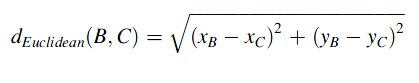
\includegraphics[scale=0.6]{images/EuclidDistance1.jpg}\\
		\end{center}
	\end{figure}
	
	The Euclidean distance is the square root of the sum of the squared differences in
	the variables’ values. Suppose B and C were positioned as $(7,6)$ and $(6,5)$ respectively.
	\begin{figure}[h!]
		\begin{center}
			% Requires \usepackage{graphicx}
			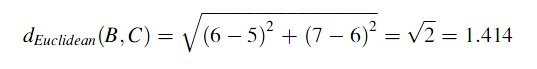
\includegraphics[scale=0.6]{images/EuclidDistance2.jpg}\\
		\end{center}
	\end{figure}
	
	This distance corresponds to the length of the line that connects objects B and C.
	In this case, we only used two variables but we can easily add more under the root
	sign in the formula. However, each additional variable will add a dimension to our
	research problem (e.g., with ten clustering variables, we have to deal with ten
	dimensions), making it impossible to represent the solution graphically.
	
	\item  The \textbf{\textit{Squared Euclidean distance}} uses the same equation as the Euclidean distance metric, but does not take the square root. In the previous example, the squared Euclidean distance between B and C is 2.
	As a result, clustering with the Squared Euclidean distance is computationally faster than clustering with the regular Euclidean distance.
	
	\item We can compute the distance between all other pairs of objects. All
	these distances are usually expressed by means of a \textit{\textbf{distance matrix}}. In this distance
	matrix, the non-diagonal elements express the distances between pairs of objects
	and zeros on the diagonal (the distance from each object to itself is, of course, 0). In
	our example, the distance matrix is an $8 \times 8$ table with the lines and rows
	representing the objects under consideration.
	\begin{figure}[h!]
		\begin{center}
			% Requires \usepackage{graphicx}
			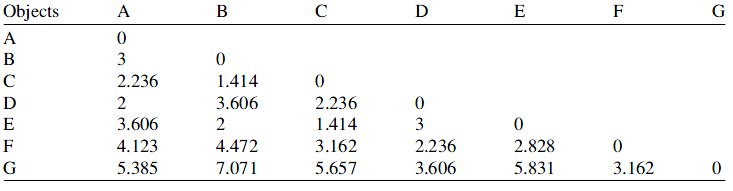
\includegraphics[scale=0.6]{images/DistanceMatrix.jpg}\\
		\end{center}
	\end{figure}
	
	\item There are also alternative distance measures: The \textbf{\textit{Manhattan distance}} or city-block distance uses the sum of the variables’ absolute differences. This is often called the Manhattan metric
	as it is akin to the walking distance between two points in a city like New York’s
	Manhattan district, where the distance equals the number of blocks in the directions
	North-South and East-West. Using the points B and C that we used previously, the manhattan distance is computed as follows:
	\begin{figure}[h!]
		\begin{center}
			% Requires \usepackage{graphicx}
			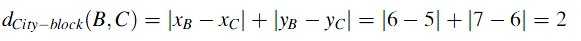
\includegraphics[scale=0.6]{images/Manhattan.jpg}\\
		\end{center}
	\end{figure}
	
	
	
	
	
	
\end{itemize}

\section{Euclidean Distance}
The Euclidean distance between two points, x and y, with $k$ dimensions is calculated as:
\[ \sqrt{ \sum^{k}_{j=1} ( x_j - y_j)^2 } \]
The Euclidean distance is always greater than or equal to zero. The measurement would be zero for identical points and high for points that show little similarity.

\subsection{Example}
Compute the Euclidean Distance between the following points:
$X = \{1,5,4,3\}$ and $Y = \{2,1,8,7\}$

\begin{center}
	\begin{tabular}{|c|c|c|c|}
		\hline
		$x_j$	&	$y_j$	&   $x_j - y_j$	&	$(x_j - y_j)^2$	\\ \hline
		1	&	2	&	-1	&	1	\\
		5	&	1	&	4	&	16	\\
		4	&	8	&	-4	&	16	\\
		3	&	7	&	-4	&	16	\\ \hline
		&		&		&	49	\\ \hline
	\end{tabular}
\end{center}
The Euclidean Distance between the two points is $\sqrt{49}$ i.e. 7.

\subsection{Euclidean Distance}
\begin{itemize}
	\item The most straightforward and generally accepted way of computing distances between objects in a multi-dimensional space is to compute Euclidean distances, an extension of Pythagoras's theorem.
	\item If we had a two- or three-dimensional space this measure is the actual geometric distance between objects in the space (i.e. as if measured with a ruler).
	\item The Euclidean distance is probably the most commonly chosen type of distance. It simply is the geometric distance in the multidimensional space. The Euclidean distance between two points, x and y, with $k$ dimensions is calculated as:
	\[ \sqrt{ \sum^{k}_{j=1} ( x_j - y_j)^2 } \]
	
	\item 
	In a univariate example, the Euclidean distance between two values is the arithmetic difference, i.e. \textbf{\textit{value1 - value2}}. In the bivariate case, the minimum distance is the hypotenuse of a triangle formed from the points, as in Pythagoras's theorem.
	\item Although difficult to visualize, an extension of the Pythagoras's theorem will give the distance between two points in n-dimensional space. 
	
	\item 
	The Euclidean distance is always greater than or equal to zero. The measurement would be zero for identical points and high for points that show little similarity.
%	\subsection{Squared Euclidean Distance}
%	The Squared Euclidean distance between two points, x and y, with $k$ dimensions is calculated as:
%	\[ \sum^{k}_{j=1} ( x_j - y_j)^2  \]
\item	The Squared Euclidean distance may be preferred to the Euclidean distance as it is slightly less computational complex, without loss of any information.
\end{itemize}
%======================================================================================= %

\noindent \textbf{Euclidean Distance : Worked Example}
Compute the Euclidean Distance between the following points:
$X = \{1,5,4,3\}$ and $Y = \{2,1,8,7\}$

\begin{center}
	\begin{tabular}{|c|c|c|c|}
		\hline
		$x_j$	&	$y_j$	&   $x_j - y_j$	&	$(x_j - y_j)^2$	\\ \hline
		1	&	2	&	-1	&	1	\\
		5	&	1	&	4	&	16	\\
		4	&	8	&	-4	&	16	\\
		3	&	7	&	-4	&	16	\\ \hline
		&		&		&	49	\\ \hline
	\end{tabular}
\end{center}
The Euclidean Distance between the two points is $\sqrt{49}$ i.e. 7.
%--------------------------------------------------------------------------------------%





%---------------------------------------------------------------------------%





\subsection{Squared Euclidean distance}

\begin{itemize}
\item The squared Euclidean distance is used more often than the simple Euclidean distance in order to place progressively greater weight on objects that are further apart. 


\item The Squared Euclidean distance between two points, x and y, with $k$ dimensions is calculated as:
\[ \sum^{k}_{j=1} ( x_j - y_j)^2  \]
\item The Squared Euclidean distance may be preferred to the Euclidean distance as it is slightly less computational complex, without loss of any information.
\end{itemize}


%http://www.econ.upf.edu/~michael/stanford/maeb4.pdf
%http://stn.spotfire.com/spotfire_client_help/hc/hc_distance_measures_overview.htm

%=========================================== %


\subsection{Manhattan (City Block) Distance}
\begin{itemize}
\item The \textbf{City-block (Manhattan) distance} is simply the aggregrate difference across dimensions. 
\item In most cases, this distance measure yields results similar to the simple Euclidean distance. However, note that in this measure, the effect of single large differences (outliers) is dampened (since they are not squared). 

%The city-block distance is computed as: distance(x,y) = i |xi - yi|

\item 
The City block distance between two points, x and y, with $k$ dimensions is calculated as:
\[ \sum^{k}_{j=1} | x_j - y_j |  \]

\item The City block distance is always greater than or equal to zero. The measurement would be zero for identical points and high for points that show little similarity.

\item  \textbf{Example}\\
Compute the Manhattan Distance between the following points: 
$X = \{1,3,4,2\}$ and $Y = \{5,2,5,2\}$, based on four numeric variables.


\begin{center}
	\begin{tabular}{|c|c|c|c|c|}
		\hline
	&	Case $X$	&	Case $Y$	&   Difference	&	$| \mbox{Diff} |$	\\ \hline
Variable 1	&	1	&	5	&	-4	&	4	\\
Variable 2	&	3	&	2	&	1	&	1	\\
Variable 3	&	4	&	5	&	-1	&	1	\\
Variable 4	&	2	&	2	&	0	&	0	\\ \hline
		& & && 6 \\
		\hline
	\end{tabular}
\end{center}
\item The Manhattan Distance between the two points is 6.
\end{itemize}



%--------------------------------------------------------------------------------------%
\newpage
\subsection{Other Measures}
\begin{itemize}
\item When working with metric (or ordinal) data, researchers frequently use
the \textbf{\textit{Chebychev distance}}, which is the maximum of the absolute difference in the
clustering variables’ values. This distance measure may be appropriate in cases when we want to define two objects as "different" if they are different on any one of the dimensions. The Chebychev distance is computed as:
\[\mbox{distance(x,y)} = \mbox{Maximum}|x_i - y_i|\] For B and C, this result is:

\begin{figure}[h!]
	\begin{center}
		% Requires \usepackage{graphicx}
		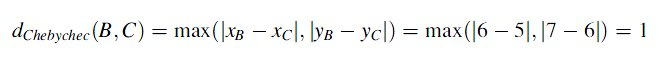
\includegraphics[scale=0.6]{images/Chebyshev.jpg}\\
	\end{center}
\end{figure}


\item \textbf{Power distance.} Sometimes we may want to increase or decrease the progressive weight that is placed on dimensions on which the respective objects are very different. This can be accomplished via the power distance. The power distance is computed as:
\[\mbox{distance(x,y)}  = (\sum_i |x_i - y_i|^p)^{1/r}\]

Parameter p controls the progressive weight that is placed on differences on individual dimensions, parameter r controls the progressive weight that is placed on larger differences between objects. If r and p are equal to 2, then this distance is equal to the Euclidean distance.

A few example calculations may demonstrate how this measure "behaves." 
\begin{itemize}
\item[$\ast$] Parameter p controls the progressive weight that is placed on differences on individual dimensions
\item[$\ast$] parameter r controls the progressive weight that is placed on larger differences between objects
\item[$\ast$] If r and p are equal to 2, then this distance is equal to the Euclidean distance.
\end{itemize}

\item \textbf{Percent disagreement.} This measure is particularly useful if the data for the dimensions included in the analysis are categorical in nature. This distance is computed as:
distance(x,y) = (Number of xi  yi)/ i
	\item There are other distance measures such as the Angular, Canberra or Mahalanobis
	distance. In many situations, the \textbf{\textit{Mahalanobis
			distance}} is desirable as this measure compensates for \textbf{\textit{multi-collinearity}}
	between the clustering variables. However, it is unfortunately not menu-accessible
	in SPSS.
\end{itemize}
%-------------------------------------------------------------------------------------------------%
\newpage
\section{Standardizing the Variables}
\begin{framed}
	{
		\large
		\noindent	Generally, it is good practice to transform the dimensions of all variables so they have similar scales.
	}
\end{framed}
\begin{itemize}
\item Note that Euclidean (and squared Euclidean) distances are usually computed from raw data, and not from standardized data. This method has certain advantages (e.g., the distance between any two objects is not affected by the addition of new objects to the analysis, which may be outliers). 
\item However, the distances can be greatly affected by differences in scale among the dimensions from which the distances are computed. 
\item 
For example, if one of the dimensions denotes a measured length in centimeters, and you then convert it to millimeters (by multiplying the values by 10), the resulting Euclidean or squared Euclidean distances (computed from multiple dimensions) can be greatly affected (i.e., biased by those dimensions which have a larger scale), and consequently, the results of cluster analyses may be very different. 
\end{itemize}




\begin{itemize}
	\item If variables are measured on different scales, variables with large values contribute
	more to the distance measure than variables with small values. 
	\item In this example, both
	variables are measured on the same scale, so that’s not much of a problem, assuming
	the judges use the scales similarly. But if you were looking at the distance between two
	people based on their IQs and incomes in dollars, you would probably find that the
	differences in incomes would dominate any distance measures.
	
	% \item (A difference of only
%	\$100 when squared becomes 10,000, while a difference of 30 IQ points would be only
%	900. I’d go for the IQ points over the dollars!).
	
	\item Variables that are measured in large numbers will contribute to the distance more than variables recorded in smaller
	numbers.
	
	\item In the hierarchical clustering procedure in SPSS, you can standardize variables in
	different ways. You can compute standardized scores or divide by just the standard
	deviation, range, mean, or maximum. This results in all variables contributing more
	equally to the distance measurement. That’s not necessarily always the best strategy,
	since variability of a measure can provide useful information. 
	
\end{itemize}
%----------------------------------------------------- %
\newpage


\section{Example: Motivation for Standardized Distance}

Let us consider measuring the distances between between two points using
the three continuous variables pollution, depth and temperature. Let us suppose that a difference of 4.1 in terms of pollution is considered quite large and unusual, while a difference of 48 in terms of depth is large, but not particularly unusual.
What would happen if we applied the Euclidean distance formula to measure distance between two cases.
\begin{center}
	\begin{tabular}{|c|c|c|}
		\hline
		% after \\: \hline or \cline{col1-col2} \cline{col3-col4} ...
		Variables & case 1 & case 2 \\ \hline 
		Pollution & 6.0 & 1.9 \\
		Depth & 51 & 99 \\
		Temp & 3.0 & 2.9 \\
		\hline
	\end{tabular}
\end{center}

Here is the calculation for Euclidean Distance:
\[ d = \sqrt{(6.0 - 1.9)^2 + (51 - 99)^2 + (3.0 - 2.9)^2}   \]
\[ d = \sqrt{16.81 + 2304 + 0.01} = \sqrt{2320.82} = 48.17 \]
\noindent The contribution of the second variable depth to this calculation is huge ,therefore one could say
that the distance is practically just the absolute difference in the depth values (equal to
$|51-99|$ = 48) with only tiny additional contributions from pollution and temperature. These three variables are on
completely different scales of measurement and the larger depth values have larger differences, so they will dominate in the calculation of Euclidean distances.


\noindent The approach to take here is \textbf{standardization}, which is is necessary to balance out the contributions, and the
conventional way to do this is to transform the variables so they all have the same variance
of 1. At the same time we \textbf{\textit{center}} the variables at their means, this centering is not
necessary for calculating distance, but it makes the variables all have mean zero and thus
easier to compare. 

\noindent The transformation commonly called standardization is thus as follows (using artificial data):
{
	\large
\[\mbox{standardized value} = \frac{\mbox{observed value - mean}}{ \mbox{standard deviation}}\]
\begin{center}
	\begin{tabular}{|c|c|c|c|c|c|c|}
		\hline
		% after \\: \hline or \cline{col1-col2} \cline{col3-col4} ...
		Variables & Case 1 & Case 2 & Mean & Std. Dev & Case 1 (std) & Case 2 (std) \\ \hline
		Pollution & 6.0 & 1.9 & 4.517	&	2.141	&	0.693	&	-1.222	\\
		Depth & 51 & 99 & 74.433	&	15.615	&	-1.501	&	1.573	\\
		Temp & 3.0 & 2.9 & 3.057	&	0.281	&	-0.201	&	-0.557	\\
		\hline
	\end{tabular}
\end{center}
}
\[ d_{std} =  \sqrt{(0.693 - (- 1.222))^2 + (-1.501-1.573)^2 + (-0.201-(-0.557))^2} \]

\[ d_{std} = \sqrt{3.667 + 9.449 + 0.127} = \sqrt{13.243} = 3.639 \]

Pollution and temperature have higher contributions than before but depth still plays the
largest role in this particular example, even after standardization. But this contribution is
justified now, since it does show the biggest standardized difference between the samples. 
\subsection{Logarithmic Transformation}
As as alternative to scaling or standardization, the user may opt to use the logarithm of a value, rather than the value itself.
%--------------------------------------------------------------------------------------%
\newpage
\section{Standardizing the Variables: SPSS Implementation}
\begin{itemize}
	\item If variables are measured on different scales, variables with large values contribute
	more to the distance measure than variables with small values.
	\item Variables that are measured in large numbers will contribute to the distance more than variables recorded in smaller
	numbers.
	
	\item In the hierarchical clustering procedure in SPSS, you can standardize variables in
	different ways. 
	\item You can compute standardized scores or divide by just the standard
	deviation, range, mean, or maximum. 
	\item This results in all variables contributing more
	equally to the distance measurement. 
	\item That’s not necessarily always the best strategy,
	since variability of a measure can provide useful information. 
\end{itemize}
\begin{figure}[h!]
\centering
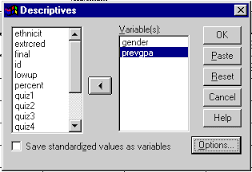
\includegraphics[width=0.5\linewidth]{spss-zscore}

\end{figure}

%-------------------------------------------------------------------------------------------------%

\section{\texttt{R} Distance Measures supported by the \texttt{dist} Function}
\begin{itemize}
	\item This is not core material for MA4128.
	\item The \texttt{dist()} function computes and returns the distance matrix computed by using the specified distance measure to compute the distances between the rows of a data matrix.
	\item 
	The distance measures supported by \texttt{dist()} are
	
	\begin{itemize}
		\item[$\bullet$] \texttt{euclidean} (but not squared euclidean directly)
		\item[$\bullet$] \texttt{maximum}
		\item[$\bullet$] \texttt{manhattan}
		\item[$\bullet$] \texttt{canberra}
		\item[$\bullet$] \texttt{binary} 
		\item[$\bullet$] \texttt{minkowski}.
	\end{itemize}
\end{itemize}



\end{document}